% !TeX root = ../main.tex
% Add the above to each chapter to make compiling the PDF easier in some editors.

\chapter{Theoretical Backgrounds}\label{chapter:introduction}
\section{Camera Model}
\subsection{Camera Intrinsic Matrix}
A camera can be consider as a linear mapping from 3D spaces to a 2D images when we ignore the lens distortion. Let us denote a point in 3D space as $\mathbf{X_{cam}} \in \mathbb{R}^{4\times1}$; the subscript \textit{cam} mean the point is located in camera coordinate frame. The 3D point $\mathbf{X_{cam}}$ is imaged in a camera view, at $\mathbf{x = PX_{cam}}$, where $\mathbf{x} \in \mathbb{R}^{3\times1}$ represent 2D points in images and $\mathbf{P} \in \mathbb{R}^{3\times4}$ is a \textit{camera projection matrix}. Fig. \ref{fig:ch1-pinhole-camera-geometry} \cite{book:multivew-geometry} illustrate the geometry relationship from 3D spaces to image spaces. Note that, for the sake of simplicity, we use homogeneous coordinate and column vector to represent a point.

\begin{figure}[htpb]
	\centering
	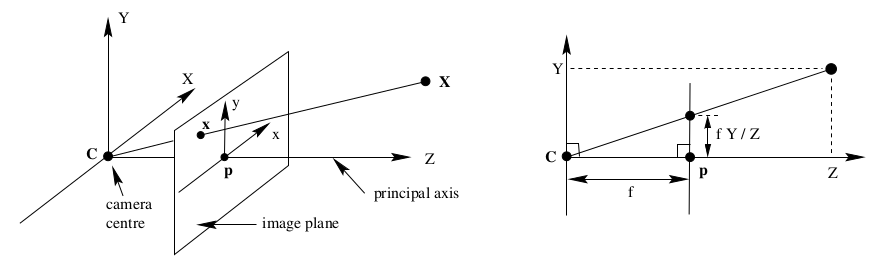
\includegraphics[width=0.7\columnwidth]{figures/ch1/pinhole-camera-geometry}
	\caption{\textbf{C} is the camera centre and \textbf{p} is the center of the image plane or called \textit{principal point}. The camera
		center is here placed at the origin of world coordinate frame. Note the image plane is placed in front of the camera center.}
	\label{fig:ch1-pinhole-camera-geometry}
\end{figure}

we can express a \textbf{basic pinhole camera model}, $\mathbf{x = PX_{cam}}$, in the following equation
\begin{gather}
\label{eq:ch1-basic-pinhole}
\begin{pmatrix} X  \\ Y \\ Z \\ 1 \end{pmatrix} \mapsto
\begin{pmatrix} fX  \\ fY \\ Z  \end{pmatrix}
=
\begin{bmatrix}
f &   &   & 0\\
& f &   & 0\\
&   & 1 & 0\\ 
\end{bmatrix}
\begin{pmatrix}
X\\
Y\\
Z\\
1\\
\end{pmatrix}
\end{gather}

Expression \ref{eq:ch1-basic-pinhole} assumes that the principle point is located at the center of image plane. Conventionally, we use the top-left or bottom-left corner of the image plane as origin. If the principle point is located at $(p_x, p_y)$ respective to a conventionally defined origin of image plane, this expression becomes
\begin{gather}
\label{eq:ch1-convention-pinhole}
\begin{pmatrix} X  \\ Y \\ Z \\ 1 \end{pmatrix} \mapsto
\begin{pmatrix} fX + Zp_x  \\ fY + Zp_y \\ Z  \end{pmatrix}
=
\begin{bmatrix}
f &   &  p_x & 0\\
& f &  p_y & 0\\
&   & 1 & 0\\ 
\end{bmatrix}
\begin{pmatrix}
X\\
Y\\
Z\\
1\\
\end{pmatrix}
\end{gather}
Now, writing
\begin{gather}
	\mathbf{K}
	=
	\begin{bmatrix}
		f &   &  p_x\\
		& f &  p_y\\
		&   & 1\\ 
	\end{bmatrix}
	\label{eq:ch1-intrinsic-matrix}
\end{gather}
then \ref{eq:ch1-convention-pinhole} has the concise form
\begin{gather}
\mathbf{x = K [I  |  0]X_{cam}} 
\end{gather}
The matrix $\mathbf{K}$ is called the \textit{camera calibration matrix} or \textit{camera intrinsic matrix} because it describe the projection from camera coordinate frame to image plane and independent from external coordinate frame, that is world coordinate frame.

\subsection{Camera Extrinsic Matrix}
In previous section, we describe a 3D point in camera coordinate frame. However, in 3D human pose datasets, 3D points $\mathbf{X}$ are mostly likely given in world coordinate frame. The two coordinate frames are related via a rotation and a translation. See Fig. \ref{fig:ch1-world-to-camera-coordinate}.

If $\widetilde{\mathbf{X}}$ is an inhomogeneous 3-vector representing the coordinates of a point in the world, and $\widetilde{\mathbf{X}}_{cam}$ represents the same point in the camera coordinate frame, then we may write $\widetilde{\mathbf{X}}_{cam} = \mathbf{R}(\widetilde{\mathbf{X}} - \widetilde{\mathbf{C}})$, where $\widetilde{\mathbf{C}}$ represents the coordinates of the camera center in the world coordinate frame, and $\mathbf{R}$ is $3 \times 3$ rotation matrix representing the orientation of the camera coordinate frame. This equation may be written in homogeneous coordinates as

\begin{gather}
\mathbf{X}_{cam}
=
\begin{bmatrix}
\mathbf{R} &  -\mathbf{R}\widetilde{\mathbf{C}} \\
0 & 1
\end{bmatrix}
\begin{pmatrix} X  \\ Y \\ Z \\ 1 \end{pmatrix}
=
\begin{bmatrix}
\mathbf{R} &  -\mathbf{R}\widetilde{\mathbf{C}} \\
0 & 1
\end{bmatrix}
\mathbf{X}
\end{gather}
Putting this together with (\ref{eq:ch1-convention-pinhole}) leads to the formula

\begin{gather}
\mathbf{x = K R [ I  |  -\widetilde{C}]X}
\label{eq:ch1-world-to-image-long}
\end{gather}
It is often convenient not to make the camera center explicit, and instead to represent he world to image transformation as $\widetilde{\mathbf{X}}_{cam} = \mathbf{R}\widetilde{\mathbf{X}} + \mathbf{t}$
In this case the camera project matrix is simply 

\begin{gather}
\mathbf{P} = \mathbf{K} [\mathbf{R} | \mathbf{t}]
\label{eq:ch1-world-to-image-convention}
\end{gather}
, where from (\ref{eq:ch1-world-to-image-long}) $\mathbf{t} = -\mathbf{R}\widetilde{\mathbf{C}}$.

The concatenated matrix $[\mathbf{R} | \mathbf{t}]$ in (\ref{eq:ch1-world-to-image-convention}) is called \textit{camera extrinsic matrix}, respect to camera intrinsic matrix. It is transformation from world coordinate frame to camera coordinate frame or called the \textit{pose} of a camera.

\begin{figure}[htpb]
	\centering
	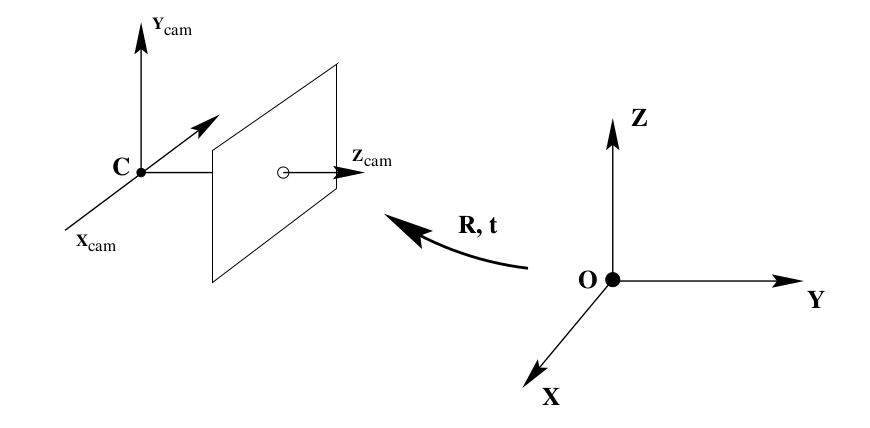
\includegraphics[width=0.7\columnwidth]{figures/ch1/world-to-camera-coordinate.png}
	\caption{The Euclidean transformation between the world and camera coordinate frames.}
	\label{fig:ch1-world-to-camera-coordinate}
\end{figure}
\section{Two-view Geometry}
\subsection{Epipolar Geometry}
Let us denote a 3D point space as  $\mathbf{X} \in \mathbb{R}^{4 \times 1}$ as shown in Fig. \ref{fig:ch1-epipolar-line}. The 3D point is imaged in two camera view, at $\mathbf{x = PX}$ by the first camera, and $\mathbf{x' = P'X}$ by the second camera, where $\mathbf{x}$ and $\mathbf{x'} \in \mathbb{R}^{3´ \times 1}$ represent 2D points in images, $\mathbf{P}$ and $\mathbf{P'} \in \mathbb{R}^{3 \times 4}$ are the camera intrinsic matrix (\ref{eq:ch1-intrinsic-matrix}). Since both points, $\mathbf{x}$ and $\mathbf{x'}$, have the same semantic meanings because they are the same point in 3D, we can, for example, fuse their features  such that each view benefits from the other view.

The epipolar geometry \cite{book:multivew-geometry} between two views is essentially the geometry of the intersection of the image planes with the pencil of planes having the baseline as axis. The baseline is the line joining the camera centers $\mathtt{C_1}$ and $\mathtt{C_2}$. In particular, for each location $\mathbf{x}$ in the first view, it helps us to determine the location of the corresponding point $\mathbf{x'}$ in the second view without having to know X.


\begin{figure}[htpb]
	\centering
	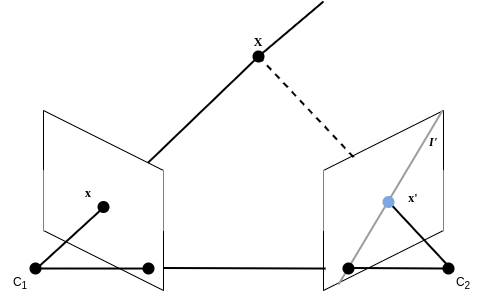
\includegraphics[scale=0.3]{figures/ch1/epipolar-line.png}
	\caption{Illustration of the point-line correspondence in two views. For an arbitrary point x in one view, the corresponding point $\mathbf{x}$ in another view has to lie on the epipolar line $\mathbf{I'}$}
	\label{fig:ch1-epipolar-line}
\end{figure}

\subsection{Fundamental Matrix}
In most cases, the 3D point $\mathbf{X}$ is unknown and, yet, we want to know where is the correspond point of $\mathbf{x}$ in the second view. We can naively search all locations in the second view, but this approach does not scale when we query more correspondent points from view 1 to view 2. Fortunately, we can compute a point-to-line relationship between two views to constrain the searching range.

The fundamental matrix is the algebraic representation of epipolar geometry. In this section, we'll only consider the case of two \textbf{calibrated} cameras. That is, the intrinsic matrices (\ref{eq:ch1-intrinsic-matrix}) and the poses (\ref{eq:ch1-world-to-image-convention}) for both cameras are known.
As illustrated in Fig. \ref{fig:ch1-epipolar-line}, assuming the camera centers do not overlap, the epipolar line $\mathbf{I'}$ corresponding to a given query pixel $\mathbf{x}$ = (x, y, 1) located on first view can be deterministically located on the other view as follows \cite{book:multivew-geometry}
\begin{gather}
\label{eq:epipolar-line}
	\mathbf{I'} = 
	[\mathbf{P'}\mathtt{C}_1]_\times \mathbf{P'} \mathbf{P}^{-1}\mathbf{x}
	= \mathbf{F}\mathbf{x}
\end{gather}
,where $[\cdot]_{\times}$ represents the skew symmetric matrix and $\mathbf{F}$ is the fundamental matrix. 

$\mathbf{x}$'s corresponding point in the second view: $\mathbf{x'}$, should lie on the epipolar line: $\mathbf{I'}^T\mathbf{x'} = 0$.


\section{Supervised Learning with Deep Convolutional Networks} 
    \subsection{Deep Convolutional Networks}
    Deep convolutional neural networks (DCNNs) have achieved state-of-the-art results in many computer
    vision tasks, such as image classification, object detection, semantic segmentation, human pose estimation, and so on. The strength is that DCNNs are able to learn richer representations than conventional hand-crafted representations.
   
    Most recently-developed 2D pose estimation networks that able to reach state-of-art performance, including Convolutional Pose Machine \cite{wei2016cpm}, Stacked Hourglass Network \cite{Newell2016StackedHN}, High-Resolution Network \cite{SunXLW19hrnet}, adopt repeative convolutional modules in their network architectures. Convolution leverages three important ideas that can help improve a machinelearning system: \textbf{sparse interactions}, \textbf{parameter sharing} and \textbf{equivariant representations} \cite{Goodfellow-et-al-2016}.
    
    \subsubsection{sparse interactions}
    A conventional 2D covolution operation is define as
    \begin{gather}
    	S(i,j) = (K * I)(i,j) = \sum_{m}\sum_{n}I(i+m,j+n)K(m,n)
    \end{gather}
    , where $K$ refer to an 2D kernel and I refer to an 2D tensor.
    One can imaging applying 2D convolution operation is like sliding a fixed window (refer to the 2D kernel) through the 2D input tensor. See Fig. \ref{fig:ch2-convolution-kernel}.
     \begin{figure}[htpb]
    	\centering
    	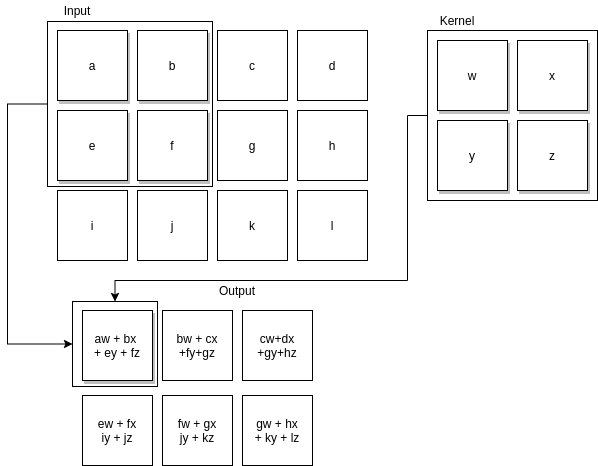
\includegraphics[scale=0.4]{figures/ch2/convolution-kernel.png}
    	\caption{ A 2D convolution. We draw boxes with arrows to indicate how the upper-left element ofthe output tensor is formed by applying the kernel to the corresponding upper-left region of the input tensor \cite{Goodfellow-et-al-2016}}
    	\label{fig:ch2-convolution-kernel}
    \end{figure}
    
    \begin{figure}[htpb]
    	\centering
    	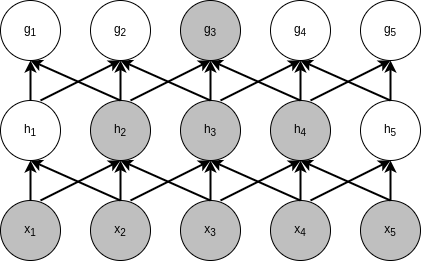
\includegraphics[width=0.5\columnwidth]{figures/ch2/receptive-field.png}
    	\caption{ A griphical demotration of a simple 3-layer CNN with only convolutional layer. Layer $\mathbf{g}$ and $\mathbf{h}$ are formed by kernel size with width 3. The receptive field of the units in the deeper layers of a convolutional network is larger than the receptive field of the units in the shallow layers. This means that even though direct connections in a convolutional net are very sparse, units in the deeper layers can be indirectly connected to all or most of the input image \cite{Goodfellow-et-al-2016}}.
    	\label{fig:ch2-sparse-connection}
    \end{figure}
    Convolutional networks typically have sparse interactions. This is accomplished by making the kernel smaller than the input. For example,when processing an image, the input image might have thousands or millions of pixels, but we can detect small, meaningful features such as edges with kernels that occupy only tens or hundreds of pixels. This means that we need to store fewer parameters, which both reduces the memory requirements of the model and improves its statistical efficiency. In a deep convolutional network, units in the deeper layers may indirectly interact with a larger portion of the input, as shown in Fig. \ref{fig:ch2-sparse-connection}. This allows then etwork to efficiently describe complicated interactions between many variables byc onstructing such interactions from simple building blocks that each describe only sparse interactions.
   
    \subsubsection{parameter sharing}
    Parameter sharing refers to using the same parameter for more than onefunction in a model. This is a direct effect of the convolution, since we apply the same kernel at every location of the input tensor, shown in Fig. \ref{fig:ch2-convolution-kernel}.
    
    \subsubsection{equivariant representations}
    In the case of convolution, the particular form of parameter sharing causes thelayer to have a property called equivariance to translation. To say a function is equivariant means that if the input changes, the output changes in the same way. Specifically, a function $f(x)$ is equivariant to a function $g$ if $f(g(x)) = g(f(x))$. In the case of convolution, if we let $g$ be any function that translates the input, that is, shifts it, then the convolution function is equivariant to $g$. In images, convolution creates a 2D map of where certain features appear in the input. If we move the object in the input, its representation will move the same amount in the output. This is useful for when we know that some function of a small number of neighboring pixels is useful when applied to multiple input locations.
    
    \subsection{Residual Learning and ResNets}
    As deeper CNNs achieve better performance on large scale datasets, researchers observe that when deeper networks are able to start converging, a degradation problem shown in  has been exposed: with the network depth increasing, accuracy gets saturated (which might be
    unsurprising) and then degrades rapidly. Unexpectedly, such degradation is \textit{not caused by overfitting}, and adding more plain layers  to a suitably deep model leads to higher training error, shown in Fig. \ref{fig:ch2-plain-network-error}.
    
     \begin{figure}
    	\centering
    	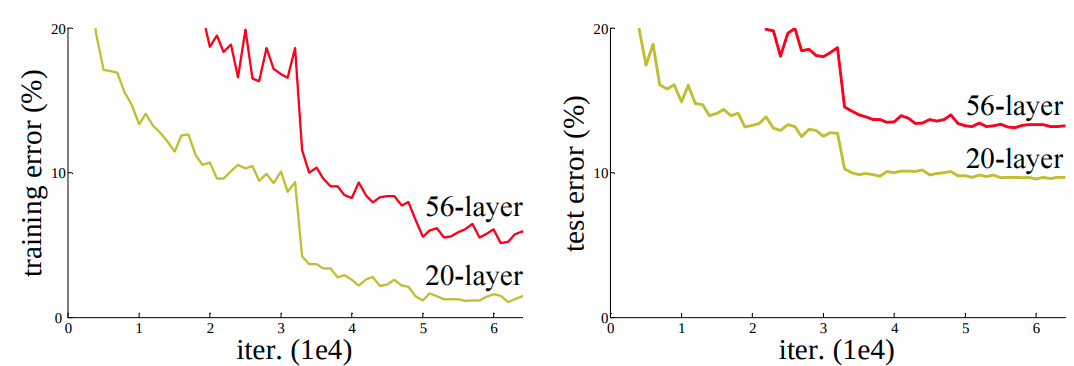
\includegraphics[width=0.7\columnwidth]{figures/ch2/evaluation-plain-deeper.png}
    	\caption{Training error (left) and test error (right) on CIFAR-10
    		with 20-layer and 56-layer “plain” networks (that
    		simply stack layers). The deeper network
    		has higher training error, and thus test error \cite{He2016Resnet}.
    	}
    	\label{fig:ch2-plain-network-error}
    \end{figure}
    
    Let us $\mathbf{H(x)}$ as an underlying mapping to be fit by a few stacked layer and $\mathbf{H(x)}$ can approximate the desired underlying function. \textit{He et al.} \cite{He2016Resnet} propose that rather than expect stacked layers to approximate $\mathbf{H(x)}$, they explicitly let these layers approximate a residual function $\mathbf{F} \coloneqq \mathbf{H(x)-x}$. The layer that learns such function $\mathbf{F}$ becomes a residual learning block Fig. \ref{fig:ch2-residual-learning-block}.The original function thus becomes $\mathbf{F(x)+x}$. They argue that although both forms should be able to asymptotically approximate the desired functions, but the form of residual learning might be easier and conduct empirical experiments supporting the argument.
    \begin{figure}
    	\centering
    	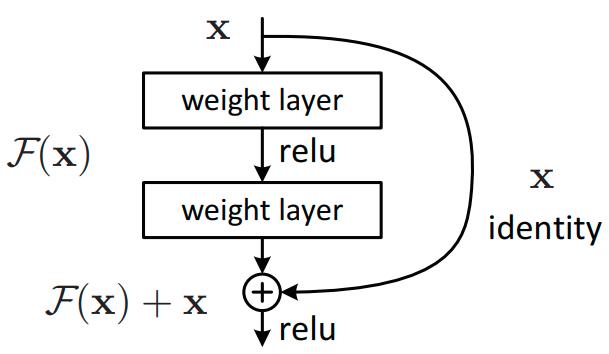
\includegraphics[width=0.5\columnwidth]{figures/ch2/residual-learning-block.png}
    	\caption{An illustration of residual block: the task for the stacked layer is to learn the residual representation $\mathbf{F(x)}$ \cite{He2016Resnet}. The curved connection is commonly called \textit{residual connections} or \textit{skip connections} interchangeably nowadays.} 
    	\label{fig:ch2-residual-learning-block}
    \end{figure}

\begin{figure}
	\centering
	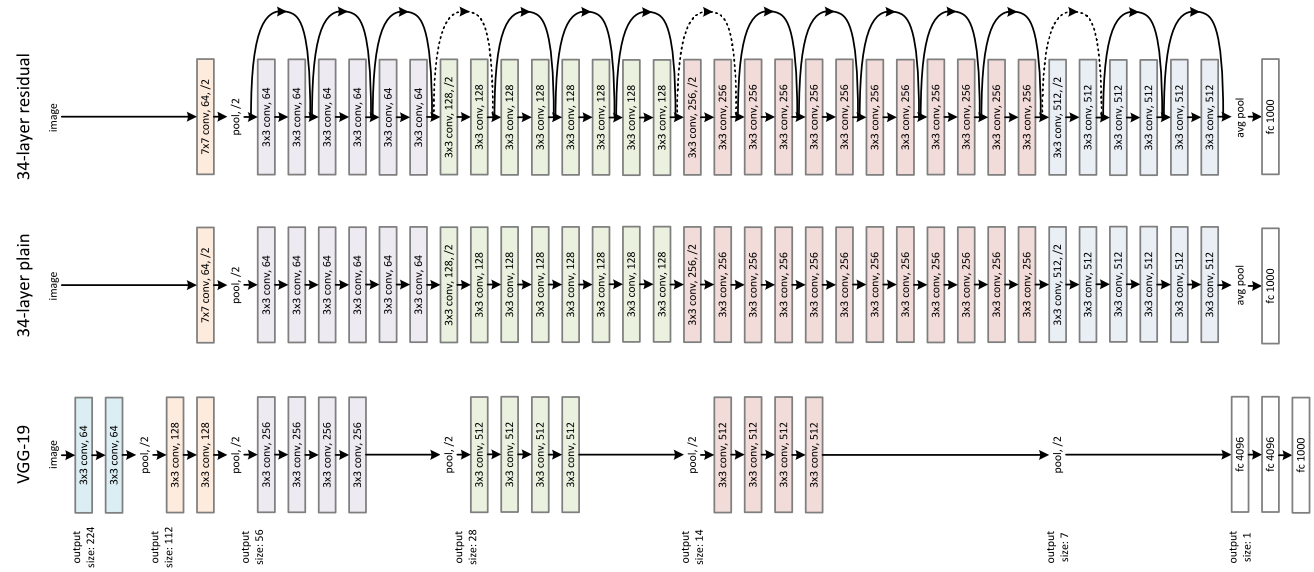
\includegraphics[width=0.8\columnwidth]{figures/ch2/resnet-architecture.jpeg}
	\caption{Example network architectures for ImageNet. 
		Top: a residual network with 34 parameter layers (3.6 billion
		FLOPs). The dotted shortcuts increase dimensions.
		Middle: a plain network with 34 parameter layers (3.6 billion FLOPs).
		Bottom: the
		VGG-19 model \cite{Simonyan15vggnets} (19.6 billion FLOPs) as a reference. \cite{He2016Resnet}} 
	\label{fig:ch2-resnet-architecture}
\end{figure}

Residual Networks or ResNets, shown in Fig. \ref{fig:ch2-resnet-architecture}, are able to reach a deeper depth and continuously improve their accuracy compare to plain networks without residual learning. Moreover, deeper ResNets outperform the previously state-of-art VGG nets \cite{Simonyan15vggnets} with significantly less parameters \cite{He2016Resnet}. One reason that explain the improved learning capabilities of ResNet might be given by a research \cite{visualloss}, that observes residual connections promote flat minimizers, shown in Fig. \ref{fig:ch2-resnet-loss}, and prevent the transition to chaotic behavior, which helps explain why skip connections are necessary for training extremely deep networks.

\begin{figure}
	\centering
	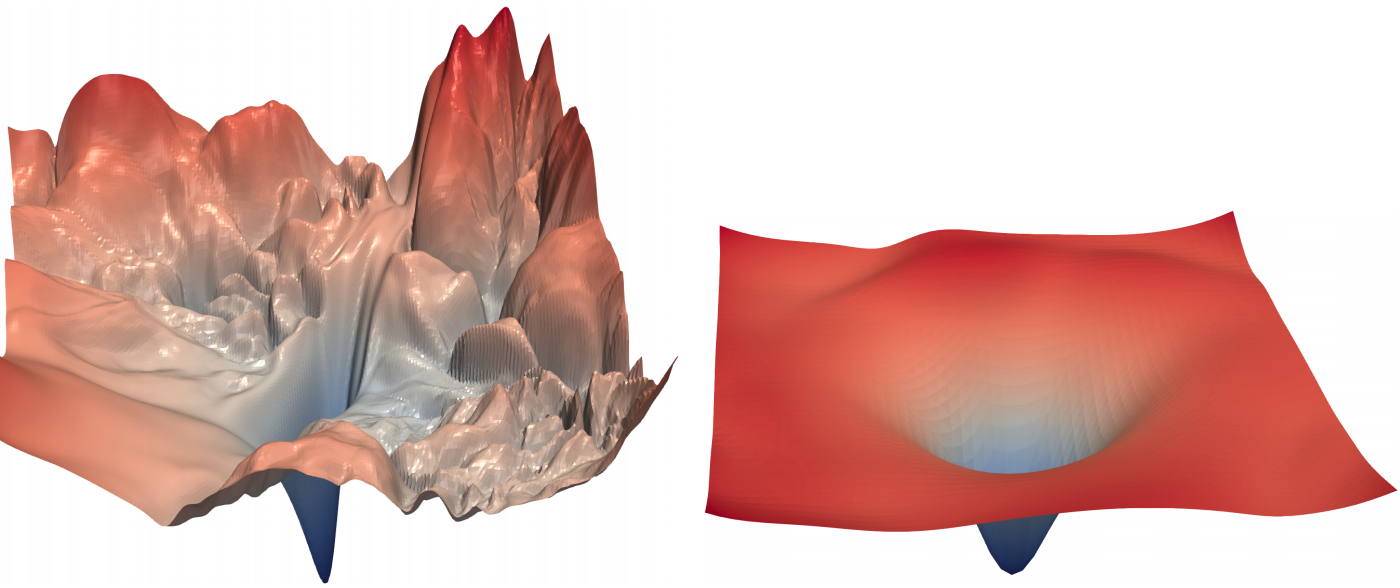
\includegraphics[width=0.8\columnwidth]{figures/ch2/resnet-loss.png}
	\caption{The loss surfaces of ResNet-56 (left) without residual connections (right) with residual connections \cite{visualloss}.} 
	\label{fig:ch2-resnet-loss}
\end{figure}
         
\subsection{3D U-Net}
3D U-Net \cite{iek20163Dunet} is a network for volumetric segmentation that learns from sparsely annotated volumetric images. See Fig. \ref{fig:ch2-3dunet-architecture} The network is based on its predecessor that takes 2D images as input, U-Net \cite{2015unet}, but takes 3D volumes as input and processes them with corresponding 3D operations, in particular, 3D convolutions, 3D max pooling, and 3D up-convolutional layers. Using 3D kernels allow the network to learn dependecies across the volumetric structures in data. 

The network is composed by two stages: contracting stage and a expansive stage (or an analysis and a synthesis path in \cite{iek20163Dunet}). In contracting stage, channel size of the input is double, but the width and height are shrink to half by mas pooling, leading the receptive field of output unit to grow fast. In expansive stage, $2\times2\times2$ transpose convolution kernels with stride two are used to double the dimiension before proceeding to the next layer. In addition, shortcut connections from layers of equal resolution in the contracting stage provide the essential high-resolution features to the synthesis stage.
\begin{figure}
	\centering
	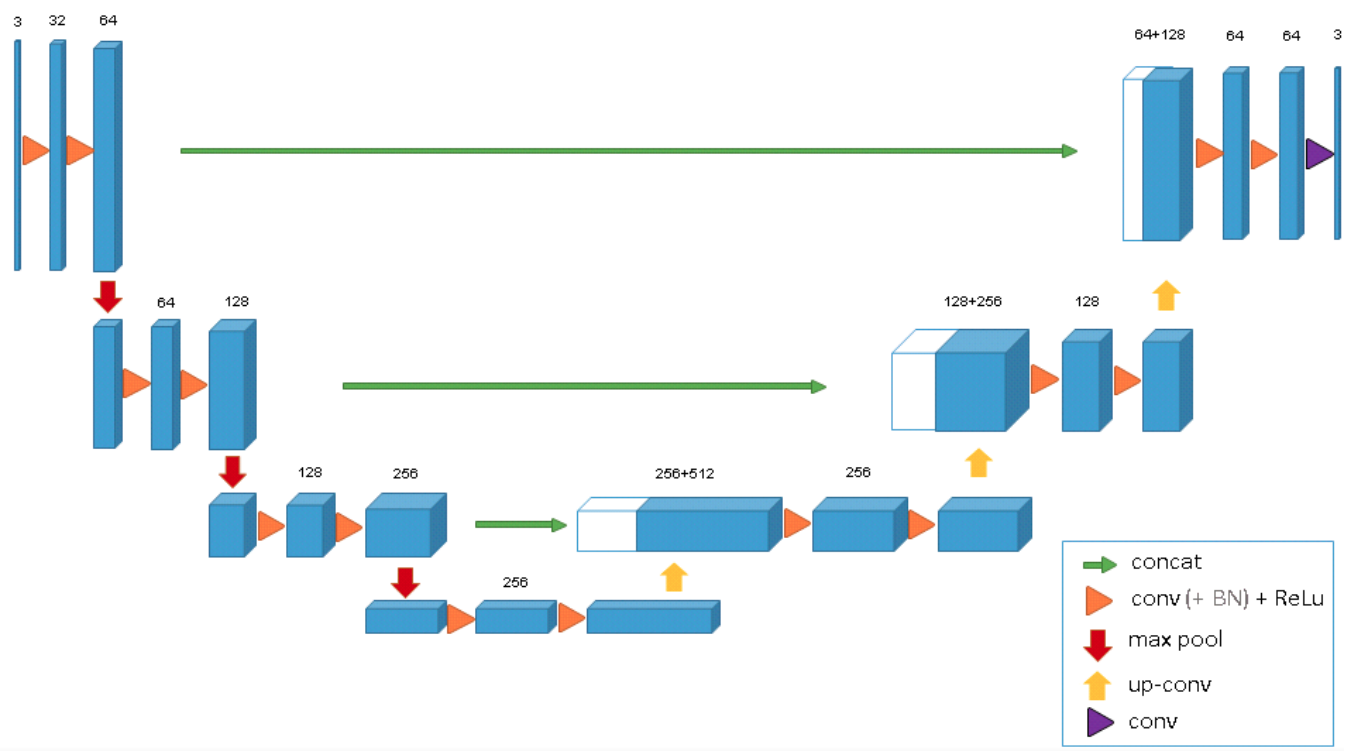
\includegraphics[width=0.7\columnwidth]{figures/ch2/3dunet.png}
	\caption{3D U-Net architecture} 
	\label{fig:ch2-3dunet-architecture}
\end{figure}

\subsection{Transfer Learning}
DCNNs proof to be successful in demonstrating high accuracy in various tasks. In practice, however, very few people train an entire DCNN from scratch (with random initialization) using the specific dataset for the task, because it is relatively rare to have a dataset of sufficient size. Instead, it is common to pretrain a DCNN on a very large dataset (e.g. ImageNet, which contains 1.2 million images with 1000 categories), and then use the DCNN either as an initialization or a fixed feature extractor for the task of interest. This is called \textit{transfer learning} 

There several tricks in conducting transfer learning:
\begin{description}
	\item[$\bullet$ DCNN as fixed feature extractor] \noindent Take a DCNN pretrained on ImageNet, remove the last fully-connected layer (this layer’s outputs are the 1000 class scores for a different task like ImageNet), then treat the rest of the DCNN as a fixed feature extractor for the new dataset. In an AlexNet, this would compute a 4096-D vector for every image that contains the activations of the hidden layer immediately before the classifier. We call these features CNN codes. It is important for performance that these codes are ReLUd (i.e. thresholded at zero) if they were also thresholded during the training of the DCNN on ImageNet (as is usually the case). Once you extract the 4096-D codes for all images, train a linear classifier (e.g. Linear SVM or Softmax classifier) for the new dataset. 
	\item[$\bullet$ Fine-tuning the DCNN] \noindent The second strategy is to not only replace and retrain the classifier on top of the DCNN on the new dataset, but to also fine-tune the weights of the pretrained network by continuing the backpropagation. It is possible to fine-tune all the layers of the DCNN, or it’s possible to keep some of the earlier layers fixed (due to overfitting concerns) and only fine-tune some higher-level portion of the network. This is motivated by the observation that the earlier features of a DCNN contain more generic features (e.g. edge detectors or color blob detectors) that should be useful to many tasks, but later layers of the DCNN becomes progressively more specific to the details of the classes contained in the original dataset. In case of ImageNet for example, which contains many dog breeds, a significant portion of the representational power of the DCNN may be devoted to features that are specific to differentiating between dog breeds.
	\item[$\bullet$ Pretrained models] \noindent  Since modern DCNNs take 2-3 weeks to train across multiple GPUs on ImageNet, it is common to see people release their final DCNN checkpoints for the benefit of others who can use the networks for fine-tuning. For example, the Caffe library has a Model Zoo where people share their network weights.
\end{description}

% Citation test~\parencite{latex}.

% \subsection{Subsection}

% See~\autoref{tab:sample}, \autoref{fig:sample-drawing}, \autoref{fig:sample-plot}, \autoref{fig:sample-listing}.

% \begin{table}[htpb]
%   \caption[Example table]{An example for a simple table.}\label{tab:sample}
%   \centering
%   \begin{tabular}{l l l l}
%     \toprule
%       A & B & C & D \\
%     \midrule
%       1 & 2 & 1 & 2 \\
%       2 & 3 & 2 & 3 \\
%     \bottomrule
%   \end{tabular}
% \end{table}

% \begin{figure}[htpb]
%   \centering
%   % This should probably go into a file in figures/
%   \begin{tikzpicture}[node distance=3cm]
%     \node (R0) {$R_1$};
%     \node (R1) [right of=R0] {$R_2$};
%     \node (R2) [below of=R1] {$R_4$};
%     \node (R3) [below of=R0] {$R_3$};
%     \node (R4) [right of=R1] {$R_5$};

%     \path[every node]
%       (R0) edge (R1)
%       (R0) edge (R3)
%       (R3) edge (R2)
%       (R2) edge (R1)
%       (R1) edge (R4);
%   \end{tikzpicture}
%   \caption[Example drawing]{An example for a simple drawing.}\label{fig:sample-drawing}
% \end{figure}

% \begin{figure}[htpb]
%   \centering

%   \pgfplotstableset{col sep=&, row sep=\\}
%   % This should probably go into a file in data/
%   \pgfplotstableread{
%     a & b    \\
%     1 & 1000 \\
%     2 & 1500 \\
%     3 & 1600 \\
%   }\exampleA
%   \pgfplotstableread{
%     a & b    \\
%     1 & 1200 \\
%     2 & 800 \\
%     3 & 1400 \\
%   }\exampleB
%   % This should probably go into a file in figures/
%   \begin{tikzpicture}
%     \begin{axis}[
%         ymin=0,
%         legend style={legend pos=south east},
%         grid,
%         thick,
%         ylabel=Y,
%         xlabel=X
%       ]
%       \addplot table[x=a, y=b]{\exampleA};
%       \addlegendentry{Example A};
%       \addplot table[x=a, y=b]{\exampleB};
%       \addlegendentry{Example B};
%     \end{axis}
%   \end{tikzpicture}
%   \caption[Example plot]{An example for a simple plot.}\label{fig:sample-plot}
% \end{figure}

% \begin{figure}[htpb]
%   \centering
%   \begin{tabular}{c}
%   \begin{lstlisting}[language=SQL]
%     SELECT * FROM tbl WHERE tbl.str = "str"
%   \end{lstlisting}
%   \end{tabular}
%   \caption[Example listing]{An example for a source code listing.}\label{fig:sample-listing}
% \end{figure}
